\documentclass[border=4pt]{standalone}
% Preámbulo común de las figuras. Cada figura es un documento standalone
% que se compila a SVG con scripts/build_figures.sh
\usepackage[utf8]{inputenc}
\usepackage{amsmath}
\usepackage{tikz}
\usepackage[american, siunitx]{circuitikz}
\usetikzlibrary{arrows.meta,calc,decorations.pathmorphing,patterns}
\tikzset{
  >={Stealth[length=2.2mm]},
  eje/.style={->, thin},
  hilo/.style={thick},
}
% Paleta común: tonos medios legibles sobre fondo claro
\definecolor{azul}{RGB}{31,94,168}
\definecolor{rojo}{RGB}{192,57,43}
\definecolor{verde}{RGB}{39,128,73}
\definecolor{naranja}{RGB}{211,120,30}
\definecolor{morado}{RGB}{125,60,152}

\begin{document}
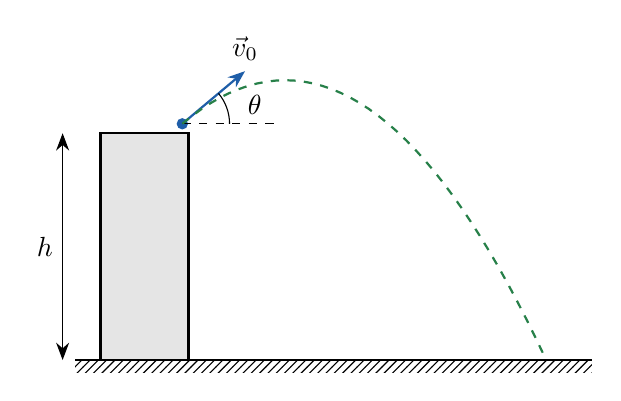
\begin{tikzpicture}[scale=0.8]
  \fill[pattern=north east lines] (-0.4,-0.2) rectangle (7.8,0);
  \draw[thick] (-0.4,0) -- (7.8,0);
  \filldraw[fill=gray!20, thick] (0,0) rectangle (1.4,3.6);
  \fill[azul] (1.3,3.75) circle (0.09);
  \draw[->, thick, azul] (1.3,3.75) -- ++(40:1.3) node[above, text=black]{$\vec v_0$};
  \draw[dashed, thin] (1.3,3.75) -- (2.8,3.75);
  \draw (2.05,3.75) arc (0:40:0.75); \node at (2.45,4.05) {$\theta$};
  \draw[dashed, verde, thick] plot[domain=0:2.222, samples=40] ({1.3+2.6*\x}, {3.75+2.2*\x-1.75*\x*\x});
  \draw[<->, thin] (-0.6,0) -- node[left]{$h$} (-0.6,3.6);
\end{tikzpicture}
\end{document}
